% ════════════════════════════════════════════════════════════════
\subsection{Termin 3}
% ════════════════════════════════════════════════════════════════

\begin{zadanie}[Zadanie 1 --- kod Huffmana dla częstości będących potęgami dwójki (15 p.)]
	Alfabet $A$ składa się ze znaków $z_1,z_2,\dots,z_n$. W~pewnym tekście $T$
	znak $z_i$ występuje $2^{i-1}$ razy dla wszystkich $i\in\{1,2,\dots,n\}$.
	Znajdź kod Huffmana dla tekstu $T$.
\end{zadanie}

Znak $z_i$ występuje $2^{i-1}$ razy, $i=1,\dots,n$ (częstości $1,2,4,\dots,2^{n-1}$).
Kluczowa obserwacja:
\[
	\sum_{j=1}^{i-1} 2^{j-1}=2^{i-1}-1\ <\ 2^{i-1},
\]
więc waga węzła scalającego pierwsze $i-1$ znaków jest mniejsza od częstości
kolejnego znaku $z_i$. Dlatego Huffman buduje ,,grzebień'': najpierw scala
$z_1$ z~$z_2$, wynik z~$z_3$, ten z~$z_4$, itd.

\begin{azfigure}
	\centering
	% Grzebień rysowany ręcznie: węzły wewnętrzne schodzą w~prawo-w~dół,
	% lewy potomek każdego z~nich to liść (krawędź 0), prawy prowadzi niżej (1).
	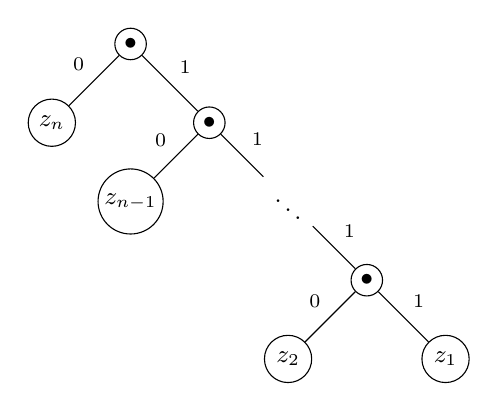
\begin{tikzpicture}[font=\small, >=stealth,
			spine/.style={circle, draw, inner sep=1pt, minimum size=4mm},
			lf/.style={circle, draw, inner sep=1.5pt, minimum size=6mm},
			lbl/.style={midway, font=\scriptsize, draw=none, fill=none}]
		% internal nodes along the spine (x = y descending)
		\node[spine]                 (r0) at (0,0)   {$\bullet$};
		\node[spine]                 (r1) at (1,-1)  {$\bullet$};
		\node[draw=none]          (rd) at (2,-2)  {$\ddots$};
		\node[spine]                 (rk) at (3,-3)  {$\bullet$};
		% leaves hanging to the left of each internal node
		\node[lf] (zn)  at (-1,-1) {$z_n$};
		\node[lf] (zn1) at (0,-2)  {$z_{n-1}$};
		\node[lf] (z2)  at (2,-4)  {$z_2$};
		\node[lf] (z1)  at (4,-4)  {$z_1$};
		\draw (r0) -- (zn) node[lbl, above left] {$0$};
		\draw (r0) -- (r1) node[lbl, above right] {$1$};
		\draw (r1) -- (zn1) node[lbl, above left] {$0$};
		\draw (r1) -- (rd)  node[lbl, above right] {$1$};
		\draw (rd) -- (rk)  node[lbl, above right] {$1$};
		\draw (rk) -- (z2) node[lbl, above left] {$0$};
		\draw (rk) -- (z1) node[lbl, above right] {$1$};
	\end{tikzpicture}
	\caption{Drzewo Huffmana dla częstości $2^{i-1}$ --- ,,grzebień''.}
\end{azfigure}

\paragraph{Słowa kodowe i~długości.}
Przyjmując konwencję ,,lewo${}=0$, prawo${}=1$'' z~rysunku:
\[
	z_n\!:\,0,\quad z_{n-1}\!:\,10,\quad z_{n-2}\!:\,110,\ \dots,\
	z_2\!:\,\underbrace{1\cdots1}_{n-2}0,\quad z_1\!:\,\underbrace{1\cdots1}_{n-1}.
\]
Długości: $\ell(z_i)=n-i+1$ dla $i\geq 2$ oraz $\ell(z_1)=n-1$ (oba najgłębsze
znaki $z_1,z_2$ na poziomie $n-1$). Sprawdzenie Krafta:
$2\cdot 2^{-(n-1)}+\sum_{i=3}^{n} 2^{-(n-i+1)}=2^{-(n-2)}+\big(1-2^{-(n-2)}\big)=1$.

\clearpage
\begin{zadanie}[Zadanie 2 --- rozdział czekolady (15 p.)]
	Kostka czekolady o~wadze $2n$ dkg spadła na podłogę i~połamała się na wiele
	kawałków, z~których żaden nie waży więcej niż $1$ dkg. Zaprojektuj algorytm
	o~liniowej złożoności obliczeniowej, który rozdziela te kawałki pomiędzy $n$
	dzieci tak, że każde dziecko dostaje kawałki o~sumarycznej wadze co najmniej
	$1$ dkg. Udowodnij, że Twój algorytm jest poprawny.
\end{zadanie}

Kostka waży $2n$ dkg, połamana na kawałki, każdy $\leq 1$ dkg; rozdzielamy je
$n$ dzieciom tak, by każde dostało $\geq 1$ dkg.

\paragraph{Algorytm (liniowy).}
Przeglądamy kawałki w~dowolnej ustalonej kolejności. Dla dziecka
$j=1,\dots,n-1$ dokładamy kolejne kawałki, dopóki jego suma nie osiągnie $\geq 1$
dkg, po czym przechodzimy do dziecka $j+1$. Wszystkie pozostałe kawałki oddajemy
dziecku $n$. Każdy kawałek dotykamy raz: czas $\BO(\#\text{kawałków})$, liniowy.

\paragraph{Poprawność.}
Gdy dziecko $j<n$ kończymy obsługiwać, jego suma $t_j$ spełnia $1\leq t_j<2$:
przed ostatnim kawałkiem było $<1$, a~kawałek dokłada $\leq 1$. Stąd pierwszych
$n-1$ dzieci zużywa $\sum_{j<n} t_j<2(n-1)$ dkg, więc dla dziecka $n$ zostaje
\[
	R=2n-\sum_{j<n} t_j\ >\ 2n-2(n-1)=2\ \geq\ 1\ \text{dkg}.
\]
Zatem każde z~$n$ dzieci dostaje $\geq 1$ dkg --- algorytm nie ,,zacina się''
przed obsłużeniem wszystkich. $\qed$

\clearpage
\begin{zadanie}[Zadanie 3 --- stacje przekaźnikowe (DP) (15 p.)]
	Firma ,,Głuchy Telefon'' buduje stacje przekaźnikowe wzdłuż autostrady A44
	o~długości $M$ km. Jest $n$ możliwych lokalizacji, leżących w~odległościach
	$m_1<m_2<\dots<m_n$ od początku autostrady (wszystkie przy autostradzie).
	Koszt budowy stacji w~lokalizacji $i$-tej to $k_i>0$, $i\in\{1,\dots,n\}$.
	Stacje trzeba wybudować tak, by z~każdego punktu autostrady było nie dalej niż
	$k$ km do najbliższej stacji. Podaj efektywny algorytm programowania
	dynamicznego obliczający najmniejszy całkowity koszt inwestycji i~oszacuj jego
	złożoność obliczeniową.
\end{zadanie}

Autostrada $[0,M]$, możliwe lokalizacje w~$m_1<\dots<m_n$, koszty $k_i>0$.
Stacja w~$m_i$ obsługuje punkty w~zasięgu $k$, czyli przedział $[m_i-k,\,m_i+k]$.
Wybieramy podzbiór lokalizacji o~minimalnym koszcie, którego przedziały pokrywają
całe $[0,M]$.

\paragraph{Programowanie dynamiczne.}
Niech $D[i]$ to minimalny koszt zbioru stacji, w~którym stacja $i$ jest
\uemph{najdalej wysuniętą} wybraną stacją, a~odcinek $[0,\,m_i+k]$ jest w~pełni
pokryty (bez luk). Wtedy
\[
	D[i]=k_i+
	\begin{cases}
		0, & m_i-k\leq 0 \quad(\text{stacja $i$ pokrywa początek}),\\[2pt]
		\displaystyle\min_{\substack{j<i\\ m_j+k\,\geq\, m_i-k}} D[j], & \text{w~przeciwnym razie,}
	\end{cases}
\]
gdzie warunek $m_j+k\geq m_i-k$ (tj.\ $m_i-m_j\leq 2k$) gwarantuje, że zasięg
poprzedniej stacji $j$ styka się z~zasięgiem $i$ --- nie powstaje luka. Gdy oba
przypadki są możliwe, bierzemy mniejszy; gdy żaden --- $D[i]=\infty$.
Odpowiedzią jest
\[
	\min_{\,i:\ m_i+k\,\geq\, M} D[i]
\]
(jeśli zbiór jest pusty, pokrycie jest niewykonalne).

\paragraph{Złożoność.}
Dla każdego $i$ minimalizujemy po~$j<i$: $\BO(n^2)$. Ponieważ lokalizacje są
posortowane, a~warunek $m_i-m_j\leq 2k$ jest monotoniczny, można utrzymywać
minimum przesuwanym oknem i~zejść do $\boxed{\BO(n)}$ (po $\BO(n\log n)$ na
sortowanie, jeśli dane nieposortowane).

\clearpage
\begin{zadanie}[Zadanie 4 --- obiekt majoryzujący (dziel i~zwyciężaj) (15 p.)]
	Tablica $A$ zawiera $n$ obiektów, które nie są liczbami (np.\ małe pliki
	tekstowe). Nie jest dla nich zdefiniowana relacja $>$, ale zdefiniowana jest
	równość (sprawdzana w~czasie stałym), oznaczająca identyczność obiektów.
	Mówimy, że tablica $A$ ma \emph{obiekt majoryzujący} $M$, jeśli więcej niż
	połowa obiektów jest równa $M$. Podaj algorytm typu ,,dziel i~zwyciężaj''
	o~złożoności $\BO(n\log n)$, który rozstrzyga, czy $A$ zawiera obiekt
	majoryzujący, i~jeśli tak --- zwraca go.
\end{zadanie}

Tablica $A[1\ldots n]$ obiektów z~samą relacją równości (sprawdzaną w~$\BO(1)$);
$M$ \uemph{majoryzuje}, gdy występuje $>n/2$ razy.

\paragraph{Algorytm.}
\begin{itemize}[nosep]
	\item \textbf{Baza:} dla $n=1$ zwróć ten jeden obiekt.
	\item \textbf{Dziel:} podziel $A$ na połowy $L,R$ i~rekurencyjnie wyznacz ich
	      kandydatów na majoryzujący: $c_L,c_R$ (lub ,,brak'').
	\item \textbf{Połącz:} jeśli obiekt majoryzuje całe $A$, to majoryzuje co
	      najmniej jedną połowę (gdyby w~obu występował $\leq$ połowy, łącznie
	      miałby $\leq n/2$). Wystarczy więc sprawdzić $c_L$ i~$c_R$: przeglądając
	      $A$ raz, zlicz wystąpienia każdego z~nich i~zwróć tego, który występuje
	      $>n/2$ razy (jeśli żaden --- ,,brak'').
\end{itemize}

\paragraph{Złożoność.}
$T(n)=2T(n/2)+\BO(n)=\boxed{\BO(n\log n)}$.
\begin{remark}
	Ten sam problem (przy samej równości) rozwiązuje liniowo głosowanie
	Boyera--Moore'a, ale zadanie wymaga schematu ,,dziel i~zwyciężaj''.
\end{remark}
